Rather than be built as a monolithic block, CowHub has a number of small, modular components that serve different purposes and form a complete system; CowHub is a system of loosely-connected micro-services. Each and every component is deployable separately, having been built and tested independently and corresponds to a source repository on GitHub. Each component can be dependent on other services in the system, but these are mocked during the testing stage and implemented fully in production. For an overview of all important components, see Figure \ref{fig:structure}.

\begin{sidewaysfigure}
  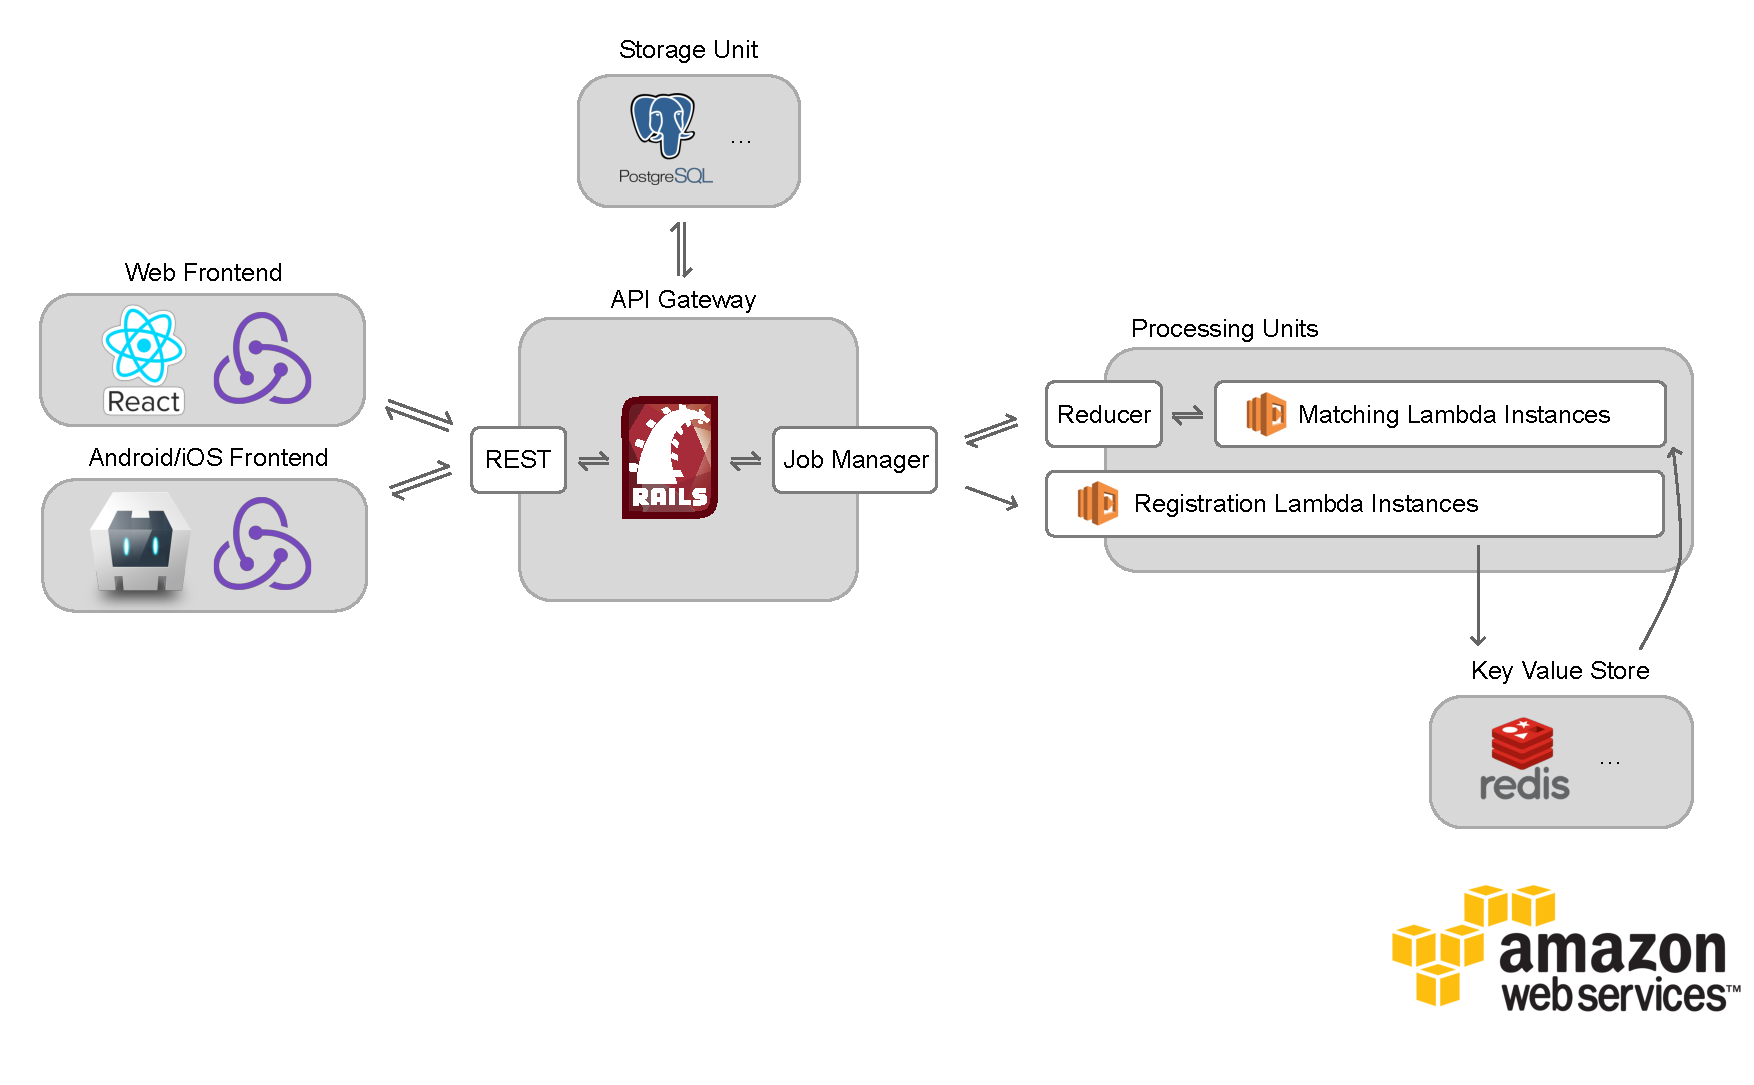
\includegraphics[width=\textwidth]{sketch/structure.pdf}
  \caption{The structure of CowHub}
  \label{fig:structure}
\end{sidewaysfigure}

CowHub uses Amazon Web Services (AWS) for a scalable, robust and stable cloud solution. For this project, the used services include IAM, CloudFront, Route 53, VPC, EC2, S3, RDS, Lambda, ElastiCache and API Gateway\footnote{This will later be referred to as Amazon API Gateway for disambiguation.}. The use of each service will be explained further in the following report.

The report proceeds with respect to the components of the project.

\subsection{Persistent Data Storage}
Persistent storage for the application is built on top of Amazon Relational Database Service (RDS) and Amazon Simple Storage Service (S3). PostgreSQL has been chosen to be the engine for the database service. The database unit aims to provide a simple, scalable and cloud-based database interface for our other services to use.

RDS has been chosen because it is an easy solution to a resizable and scalable database, and provides features such as duplication~\cite{rds}. By employing RDS we could focus more on the application that we are building and pay little to no attention to the time-consuming database administrative tasks.

S3 is used to hold all file and blob data. It has been chosen because of its persistent, simple, durable infrastructure and more importantly, its integration with other Amazon and CowHub services~\cite{s3}.

The database is to store the following:

\begin{enumerate}
	\item The information about farm and farmers. 
	\item The information about registered cattle, including the herd number, (optionally) the name, the owner, the birthdate, and most importantly the sample image(s) of its muzzle for identification uses.
	\item The login details of registered farmers. Farmers will need to log in to be able to input and review the cattle data.
	\item The match results. Every match job will be assigned a job ID and the result will be stored into the database. These match results will be useful in the future as statistics.
	\item Other data for the system to run smoothly (including session tokens etc.). 
	% TODO: more stuff about databases
\end{enumerate}

The database unit is only accessible through the API Gateway\footnote{Images are encoded in Base64 format before transfer (as a string).}.

\subsection{API Gateway}
The API Gateway (API) can be thought of as the centre of the system, and is written in Ruby on Rails (RoR). RoR has enabled us to prototype and implement the component in an elegant and efficient manner; its seamless integration with Rspec has also allowed us to test the component more efficiently\footnote{Nearly all sub-components have automated tests and are integrated with the continuous integration and delivery system.}.

The API has two most important subcomponents:

\begin{enumerate}
	\item A REST API for communication with the front-ends.
	\item A Job Manager for communication with the headless computational unit.
\end{enumerate}

The REST API mainly handles the following:

\begin{enumerate}
	\item Account management. A user (farmer) needs to be able to manage his/her personal data, change passwords and etc.
	\item Cattle management. A user (farmer) needs to be able to create/edit/delete information about a cattle and upload/update/delete images for a cattle. 
	\item Session management. The API handles sessions through tokens in a unified manner for all front-ends that require user login as REST API is stateless.
	% TODO: more stuff about our API
\end{enumerate}

We have a standardised URL schema for the API that allows us to develop the component more efficiently.

The Job manager is the more interesting part. There are two different types of jobs:

\begin{enumerate}
	\item Cattle registration job. For this type of job, an anonymous job is created (the result is not saved into the database). This is required because we do not match image with image; instead we used an edge descriptor to mathematically describe the muzzle of a cattle. The registration job is to deal with the descriptor generation so that we do not have to calculate the descriptor every time it is required.
	\item Cattle matching job. A job ID is required for this type of job as 1) we need to be able to track the status of the ongoing job and 2) we need to save the match result for statistical purposes. The process, roughly, includes (in the following order):
	\begin{enumerate}
		\item Generate the descriptor for the image to be matched.
		\item Divide the database of images into chunks with size $N$\footnote{A predefined value. For the proof of concept we have chosen 25.}, label each chunk with an ID $\text{id}_i$. This will be submitted by the API, but carried out by the Job Assignment Lambda.
		\item For each chunk with ID $\text{id}_i$, forward the ID, the job ID and the image descriptor to the headless computational unit (the Matching Lambda) and wait for a best match within the chunk to be handed back to the cache accordingly (details in~\ref{sec:lambda}).
		\item Retrieve the best match from the cache service and forward it back to the requester.
	\end{enumerate}
\end{enumerate}

Based on our statistics, step (a) normally takes a half to one second, and every pairwise match in step (c) takes about 5 to 25 milliseconds\footnote{This is due to the resizing and normalisation done prior to the match.}. That is, ignoring the network and IO delays, a match will take about $T = N * t_m / 1000 + t_d / 1000$ seconds to complete, where $t_m \in [5, 40]$ (including the time for de/serialisation) and $t_d \in [500, 1000]$. In this reasoning our computation time can be thought of as upper bounded by $Nc$, where $c$ is a constant, which is totally size-agnostic, because it is based on the assumption that we would always have $\lceil M / N \rceil$ computational units at our disposal. This rational implies that, in theory, the computation time does not generally grow with respect to the number of images in our database\footnote{In practice it does - because we cannot ignore the time consumed for IO actions.}.

\subsection{Key Value Store}
A cluster of Redis servers is employed through Amazon ElastiCache service. 

For performance reasons it has been decided that we use a key value store for concurrent and lively access for the descriptor of an image. This store is to be accessed very frequently and as only a small piece of data is being extracted at once it seemed inappropriate to be using a database. Another reason that a key value store is used, as opposed to accessing the descriptor directly from the database unit is data separation - the only place that this data is being accessed is the headless computational unit and nothing more. Also, as suggested before, the database unit is only accessible through the API, and any access directly from other components would break the promise; alternatively, to access the descriptors through the API would introduce significant (and unnecessary) burden to the API itself and result in great performance problems.

\subsection{Headless Computational Unit}
\label{sec:lambda}
The processing is built on top of AWS Lambda services. The headless computational unit supports three different kinds of jobs: registration, job assignment and matching, as suggested before. A call to the headless computational unit will cause a Lambda calculation unit (Lambda) to be spawned~\cite{lambda}. Lambda processes are running concurrently, and they are not necessarily on the same machine\footnote{It can be thought of as Actors - universal primitives for concurrent computation. Similar constructs implementation include \textit{Akka} for Scala.}.

The three different kinds of the Lambda processes include:

\begin{enumerate}
	\item Registration Lambda. This is a one way communication. The caller (the API) calls the headless computational unit, causing a Registration Lambda to be spawned. This Lambda process will run to the end (the generation of the descriptor of an image) and then store it into the Key Value store.
	\item Job Assignment Lambda. The API would have to submit the image to be matched and trigger the Job Assignment Lambda. This Lambda will slice the existing descriptors into $n=\lceil M / N \rceil$ chunks, and invoke $n$ Matching Lambdas asynchronously.
	\item Matching Lambda. The caller will need to call the headless computational unit with the job detail, and the Matching Lambda will run the match for $N$ images as discussed before. This process is completely concurrent. Upon completion of the process, the Lambda will write the best match within a batch of $N$ images back to the cache service if the match is better than the current one in the cache.
\end{enumerate}

The process of matching is similar to that of MapReduce, and so is the implementation. The only difference, through the use of AWS Lambda, is that we do not provision or administer the servers ourselves - the computational units are spawned ad hoc and only whenever needed.

\subsection{Mobile and Web Front-ends}

Our plan when designing the front-end was to support a number of platforms, ideally sharing the same codebase while still providing a native experience to the user. The requirement is to provide a mobile frontend allowing a user to photograph, geolocate and identify cattle, and an administrative web interface to manage user accounts and input further cattle information. 

The front-ends we implement are all stateless, meaning that they will run independently. Another important implication of our system design where the front-ends all communicate through the same globally accessible APIs is that users can develop their own front-ends easily, should they feel that the provided front-ends are not for their taste.

\subsubsection{Web Frontend}
The Web front-end is implemented using React.js and Redux, which are JavaScript libraries used to build user interfaces. These libraries allow us, during development, to modify the WebView style and content and view the changes without the need to re-render a page. This allows to perform a number of action:

\begin{itemize}
	\item modify the state of the application to display a particular components (registration form, deleting form, etc...)
	\item display a modified information without the need to re-render the whole page
	\item the possibility to navigate between different pages and storing the information, so that there is no need to make a server call every time we open a specific page
\end{itemize}

\subsubsection{Mobile Frontends}

Both the mobile and web frontends access the same API provided by the backend and have many common actions, so in order to share and reuse as much code as possible we implement the mobile interface using the same web technologies as the web frontend, using React and Redux running inside a WebView which is wrapped into a standalone application by Apache's Cordova framework. This is known as a "hybrid" structure, since the same application will run unmodified in a browser as well as standalone applications on mobile devices. This approach presents us with a number of advantages:

\begin{itemize}
	\item all of the high-level application logic is written in JavaScript, giving the same behaviour cross-platform, meaning that we can start the development without any prior platform-specific knowledge;
	\item agile development of the application is allowed with extremely quick prototyping and deployment  - the application can be tested and modified in a browser on a desktop, rather than having to compile and run a native application in an emulator or on a physical device;
	\item most of the Node.js libraries are made available for use: React.js and Redux as used in the web frontend for example, as well as HTML5 libraries for geolocation and ondevice image manipulation;
	\item allows us to support a large number of platforms quickly, since Cordova is available on almost all modern mobile operating systems;
\end{itemize}

Downsides include:

\begin{itemize}
	\item poor performance from extensive use of Webview. Web components will render much more slowly than using OS provided native components. The lack of OS optimisation results in increased battery consumption;
	\item access to low-level and platform dependant features are limited and involve extensive use of plugins to Cordova, these cannot be tested in the browser, are often poorly documented and can be tricky to manage, as opposed to OS provided APIs which can often be easily dropped in. HTML5 features are dependant on the system browser providing the Webview. Android suffers from a large amount of fragmentation, with many devices shipping different Android versions and browsers. This means it is difficult to guarantee that the application will work on a certain device, whereas with a native application the systems package installer will be able to determine if a device is compatible. HTML5 features are also not available while the application is running in the background, since the Webview is paused. This can affect access to features such as geolocation;
	\item difficulty in maintaining clean, reusable, easily testable code. Web applications tend to often mix core logic with the view, making it difficult to reuse in other parts of the application and to isolate components to test;
	\item it can be difficult to provide a "native" experience, since system provided components need to be recreated with web elements;
\end{itemize}



We quickly realised that the view rendering code for the mobile interface would have to differ from the web interface. Users on mobile platforms expect content to be spread over a number of concise pages, with clean and smooth page transitions and navigation, as opposed to desktop web interfaces, which tend to have more screen real estate available so more content is displayed with fewer page clicks preferred. React-router, which we use for navigation on the web front-end, does not provide page transitions out of the box.

\subsubsection{Initial mobile application prototype}

Initially we prototyped an application to be able to demonstrate the basic functionality of our API. A simple web application was written using html and JavaScript, with Android style components provided by a styling framework called Framework7. The simple code style of this application allowed us to produce a fully working prototype in just over a week. However for a number of reasons this branch would prove to be a dead end. 

Firstly all the logic was contained within a single js file, combined with jQuery calls which were updating the view. Even this simple application was proving difficult to maintain and to add additional features. This would have also reduced it's future testability. 

Secondly this version used different frameworks to our web front-end, which was already being developed using React and Redux. This meant that we were having to implement common features twice, whereas we wanted to be able to share code between the two front-end efforts.

Finally Framework7 proved to be lacking in respect to supporting multiple platforms at once. We wanted to support both Android and iOS with the same code base, which would have meant developing a whole new application.

This prototype became the predecessor to our current front-ends.

\subsubsection{Current mobile applications}


Our mobile front-ends attempt to simulate a "native" interface using the Onsen UI framework. Onsen provides a navigator class that renders pages and provides navigation between them, but most crucially also provides react components which are styled as native components. Onsen contains components styled for both Android and iOS, and after detecting what OS the Webview is running in, applies the appropriate style. When a future release of Onsen supporting Windows Phone is released, a third port of the mobile frontend will be trivial to implement.


The Onsen navigator component does not currently support controlling navigation through Redux, so our frontends provide a wrapper for the navigator, allowing us to achieve reliable navigation dispatched through redux actions. 

Our front-ends are written in ES6 JavaScript, allowing clearer code style, proper classes and native modules. This makes it easy to define modules which can be easily tested and reused. We use the babel transpiler and Webpack to produce ES5 code that will run in current phone browsers since ES6 support is limited. 
 
One of the largest challenges was implementing the camera view. While Cordova ships with a camera plugin, it simply calls the system camera, meaning that you are not able to overlay custom text and graphics such as a muzzle overlay for lining up an image of cattle correctly. If we had written a native application for Android, the functionality could have been easily achieved by building a custom camera component. Cordova also allows custom OS plugins to be added, so with some difficulty we could have imported a custom camera application. However this approach would mean writing a custom camera ourselves for each platform we wish to support. This would have been time-consuming to implement and maintain given the time-constraints of the project. Ultimately we solved this issue by using an opensource\footnote{The author has added a morality clause to a standard MIT license, restricting use in applications which are considered illegal}  augmented reality plugin called ezAR. 

EzAR is a collection of packages amongst which there is a video overlay and a snapshot plugin. The video overlay activates the camera and displays the live camera feed behind the Webview. We are able to produce a custom camera view using react components, and use a modified Onsen to create transparent pages so the camera view can be seen. The snapshot plugin was originally designed to allow you to take screenshots of an application by grabbing an image from the camera and rendering the Webview on top of the image. By using a special debugging flag the plugin will return only the camera image. This means we can re-purpose the plugin as full custom camera. In the future native camera plugins can simply be slotted in in it's place.

By using Redux we are able to separate the core application logic from the view, opening up the ability to share logic with the web front-end and since the reducers are all pure functions this logic is easy to test.


In general despite expected difficulties with access to low level features, the hybrid application approach has allowed us to implement a well structured easily extensible front-end withing the tight time constraints of this project.


\subsection{Implementation Difficulties And Comments}

% TODO: finish the implementation difficulties section

\subsubsection{Headless Computational Unit}

One serious issue here is performance, especially in the thinning process\footnote{Zhang-Suen thinning algorithm.} as the computational task is quite substantial. In this special case, it is required to inline C++ code as opposed to having pure Python code for the thinning iteration\footnote{The inline version runs within 600ms with IO whereas the pure Python version just times out after 10 seconds.}. The recommended approach is to use \texttt{weave} from \texttt{scipy} to inline the small piece of code. However this has proven to be not so easy: Amazon Lambda has a (code) package size limit of 250MB, and \texttt{scipy} itself is over 200MB - this implies that there is no way that we can use \texttt{scipy}.

It has come to us that since we only need to use \texttt{weave} and according to the official documentation, it can be installed as an independent library. Weird enough, it turns out that \texttt{weave} uses \texttt{scipy} internally - meaning that we will not be able to use \texttt{weave} at all.

The only way that's left then is to manually compile the C++ code into an object file for Python to use. Fortunately this is not too difficult: all we need to do is to run the code with \texttt{weave.inline} on a compatible machine and grab the \texttt{weave}-generated C++ file from the cache and for every platform we compile it into an object file and leave it inside the \texttt{lib} directory. This works because \texttt{weave} generates the boilerplate for seamless Python integration. After this step we would be able to replace the code with a call to the generated function in the generated module and remove the requirements for \texttt{weave} and \texttt{scipy}.

\subsubsection{Maintaining Security}

% TODO: Maintaining security comments

\subsubsection{Infrastructure Financial Constraints}

% TODO: Infrastructure financial constraints

\subsubsection{Keeping The API Gateway Performant} 

% TODO: Keeping the API Gateway Performant
